% !TeX spellcheck = en_US
% !TeX encoding = UTF-8
% !TeX root = ../thesis.tex

\chapter{Swarm Reinforcement Learning with Graph Neural Networks}
\label{ch:Architecture}
% pages: 4.26-5.68
% ~966 words
First we will introduce the policy architecture used as the base. It is designed to work with PPO and uses the latent node features of the observation for the actor and critic. This base is then expanded with a Graph Neural Network structure that allows multiple hops through a stack of message passing blocks. To support heterogeneous graphs needed for tasks like pursuit the architecture is extended to work on multiple graphs as inputs, but it retains the overarching structure. This makes both GNNs interchangeable. Most of the changes needed for heterogeneous graphs is located in the edge-, node- and global-modules.


% ~322 words
\section{PPO - Policy Architecture}
\begin{figure}[htp]
    \centering
    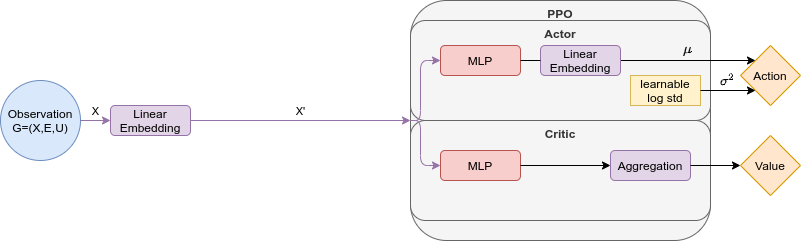
\includegraphics[width=1.0\textwidth]{figures/PPO_no_message_passing.png}
    \hspace{1cm}   
    \caption{Policy architecture used for Swarm Reinforcement Learning with Graph Neural Networks. The node features of the observation graph is the only data used. It is put into a latent dimension and then used by the PPO Network to calculate the action as a distribution and the value.}
    \label{fig:PPO_no_message_passing}
\end{figure}
Our environments can have different observations structured as a graph. For now we will talk about homogeneous graphs. Each agent $a_k$ uses information it knows about itself and what it knows about it's neighboring agents $a_i \in \mathcal{N}_k$. The specific data for each environment is described in \Cref{ch:Experiments}. Information about $a_k$ is used as the node-features for the graph. The edges $E$ describe neighborhood relations for a given $\mathcal{N}_k$. For an edge $\{v_i,v_j\} = e \in E$ edge-features on the other hand describe the individual observations from $a_x$ about the state of the agent $a_y$. \Citet{RobinRuede2021} uses a similar observation structure implicitly. Edge-features are created using an $\textup{observe()}$ function. They explicitly calculate the neighborhood for each agent that uses the policy. \par

For testing and debugging purposes, the Graph Neural Network (GNN) can be disabled. When it is, only the node-features are used. Once the observation graph is constructed, the node-features are encoded into a latent-space representation. For this embedding we use a linear layer. The Multi-Layer Perceptron (MLP) used in \Citet{RobinRuede2021} is used as an encoding step and to process each element of an aggregation group. Processing is not needed for our embedding, as our GNN is responsible for that, so a simple linear transformation is enough. \par

The learning head for Proximal Policy Optimization (PPO) is composed of the actor describing the policy $\pi$, which gets us the joint action $\textup{act} = (\textup{act}_1,...,\textup{act}_n)$ and the critic calculating the running advantage $A$. Our actor uses an MLP, followed by another linear transformation. It will reduce the dimension from the latent dimension back to the action dimension. This is then used as the mean $\mu$ for a diagonalized Gaussian distribution to support non deterministic policies. The variance $\sigma^2$ uses a learnable logarithmic standard deviation. The critic also uses an MLP with an output-dimension of 1. This defines a value per node in the graph. In \Citet{RobinRuede2021} the authors define a value for each agent. This helps to identify which agent was responsible for the reward. But this is not how the PPO Algorithm was originally designed to work for single-agent environments. Our architecture can use an aggregation to output a single value per graph. This can either be $\min(x)$, $\max(x)$, $\textup{mean}(x)$. Through exploration the agents are still able to identify over time how much an agent was responsible for a given reward. We parameterized node-wise values and graph-wise values for our approach. \par

An overview of the policy architecture as desribed above can be seen in \Cref{fig:PPO_no_message_passing}.


% ~322 words
\section{Homogeneous Message-passing GNN Architecture}
\begin{figure}[htp]
    \centering
    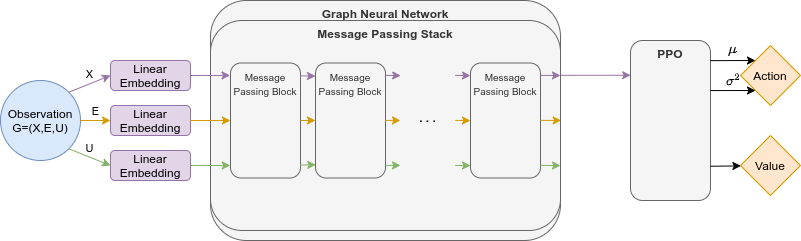
\includegraphics[width=1.0\textwidth]{figures/homogeneous_gnn.png}
    \hspace{1cm}   
    \caption{Here a GNN is added as a step before the policy architecture. The entire observation is put into a latent space and then passed through multiple message passing passes. The outputs of one pass is used as the input of the next pass. This is coordinated through the message passing stack.}
    \label{fig:homogeneous_gnn}
\end{figure}

An overview of the message passing architecture for homogeneous graphs can be seen in \Cref{fig:homogeneous_gnn}.

\begin{itemize}[noitemsep,nolistsep]
    \item Observation Embedding. Nodes, Edges and Globals.
    \begin{itemize}[noitemsep,nolistsep]
        \item No shared weights.
    \end{itemize}
    \item Robin: Basically a Message Passing like structure.
    \begin{itemize}[noitemsep,nolistsep]
        \item For a single observation group:
        \item $f(a_i) = decoder(selfObserve(a_i), \underset{j \in \mathcal{N}_i}{aggr}\ encoder(a_i, observe(a_i, a_j)))$
        \item $f(x_i) = \phi(x_i, \underset{j \in \mathcal{N}_i}{aggr}\ \psi(x_i, x_j))$
    \end{itemize}
    \item GNN composed of Stack. Stack are multiple Message Passing Blocks (a single message passing pass) in sequential order.
    \begin{itemize}[noitemsep,nolistsep]
        \item Easy to create multiple hops.
    \end{itemize}
    \item Block: 3 Modules: Edge-, Node-, Global. How they are wired. Compare that to normal message passing?
    \item Edge-Module:
    \begin{itemize}[noitemsep,nolistsep]
        \item $x_{e'} = f_e(x_v, x_u, x_e, x_g)$
    \end{itemize}
    \item Node-Module:
    \begin{itemize}[noitemsep,nolistsep]
        \item $x_{v'} = f_v(x_v, \oplus_{\{e'=(v,u)||_v\}} x_{e'}, x_g)$
    \end{itemize}
    \item Global-Module:
    \begin{itemize}[noitemsep,nolistsep]
        \item $x_{g'} = f_g(\oplus_V x_{v'}, \oplus_E x_{e'}, x_g)$
    \end{itemize}
    \item Variations/Parameter/Features:
    \item share-base:
    \item aggregation-function used in modules.
    \item use-residual-connections.
\end{itemize}

An overview of the homogeneous message passing block can be seen in \Cref{fig:message_passing_block}.

\begin{figure}[htp]
    \centering
    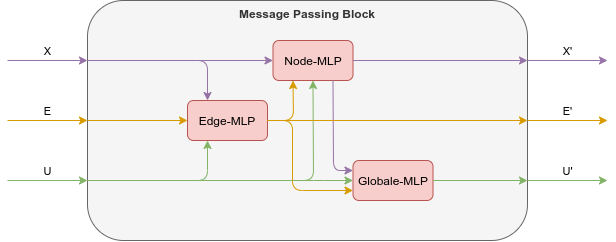
\includegraphics[width=0.75\textwidth]{figures/message_passing_block.png}
    \hspace{1cm}   
    \caption{This is a detailed view of one message passing block. It uses a edge-, node- and global-module to compute a single message passing pass.}
    \label{fig:message_passing_block}
\end{figure}


% ~322 words
\section{Heterogeneous Message-passing GNN Architecture}
\begin{figure}[htp]
    \centering
    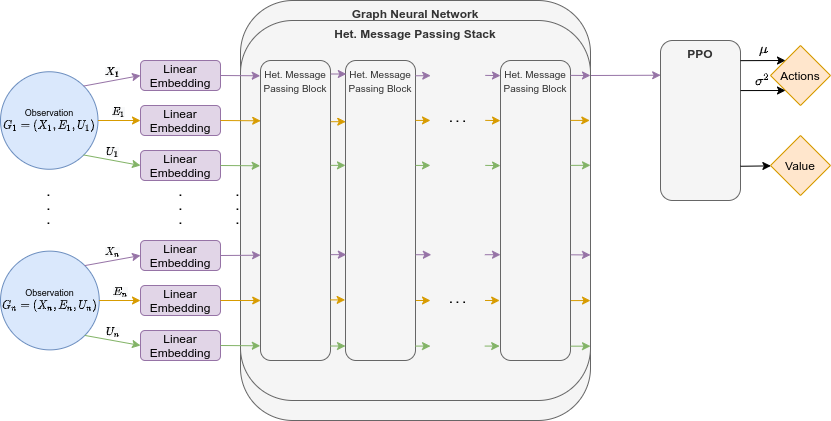
\includegraphics[width=1.0\textwidth]{figures/heterogeneous_gnn.png}
    \hspace{1cm}   
    \caption{An overview of the heterogeneous version of the architecture. The overall structure stays the same, but the input observation is now mulitple graphs. each of the input embeddings per graph is unique. The policy architecture only uses one of the note types as input.}
    \label{fig:heterogeneous_gnn}
\end{figure}

An overview of the message passing architecture for heterogeneous graphs can be seen in \Cref{fig:heterogeneous_gnn}.

\begin{itemize}[noitemsep,nolistsep]
    \item heterogeneous Graphs, MultiGraph. How the data is layed out (math!). Here shown as multiple Graphs.
    \begin{itemize}[noitemsep,nolistsep]
        \item Robin: Needed so that we have support as multiple observation groups. We use heterogeneous graphs.
        \item edge-types, node-types (PyG) => We show it using multiple graphs. (Math!)
        \item directed vs. undirected Graph
    \end{itemize}
    \item Linear Embedder for each type!
    \begin{itemize}[noitemsep,nolistsep]
        \item No shared weights. (Robin: shared weights!) why?
    \end{itemize}
    \item Stacks and Blocks are basically the same, it just now support more inputs.
    \item Edge-Module:
    \begin{itemize}[noitemsep,nolistsep]
        \item $x'_{e_i} = f_{e_i}(x_v, x_u, x_{e_i}, x_g), e_i = (u, v)$
        \item iterate: edge-types -> node-types
    \end{itemize}
    \item Node-Module:
    \begin{itemize}[noitemsep,nolistsep]
        \item $x'_{v'_i} = f_{v_i}(x_{v_i}, [\otimes_j\ \oplus_{\{e_j=(v_i,u)\}} x'_{e_j}], x_g)$
        \item iterate: node-types -> edge-types
    \end{itemize}
    \item Global-Module:
    \begin{itemize}[noitemsep,nolistsep]
        \item $x'_{g} = f_g([\otimes_j\ \oplus_{V_j} x'_{v\in V_j}], [\otimes_k\ \oplus_{E_k} x'_{e\in E_k}], x_g)$
    \end{itemize}
    \item neighbor-aggregation-types concat(aggr()), aggr(aggr())
    \begin{itemize}[noitemsep,nolistsep]
        \item concat(aggr()) (Robin): More expressive, more expensive.
        \item aggr(aggr()) (Robin): less expressive, less expensive. In multi-pursuit: hard to distinguish agents from evaders.
    \end{itemize}
\end{itemize}

An overview of the heterogeneous message passing block can be seen in \Cref{fig:heterogeneous_message_passing_block}.

\begin{figure}[htp]
    \centering
    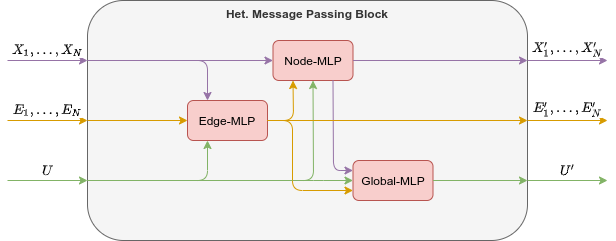
\includegraphics[width=0.85\textwidth]{figures/heterogeneous_message_passing_block.png}
    \hspace{1cm}   
    \caption{Also the structure of the message passing block stays similar. Now the three blocks take all the nodes, edges and global-features of all graphs as input and as output.}
    \label{fig:heterogeneous_message_passing_block}
\end{figure}
